\documentclass[utf8]{ctexart}
\usepackage[margin=1in]{geometry}
\usepackage{setspace}
\usepackage{hyperref}
\usepackage{graphicx}
\usepackage{booktabs}
\usepackage{longtable}
\usepackage{amsmath}
\usepackage{tikz}
\usetikzlibrary{arrows.meta,positioning,shapes.geometric}
\usepackage{float}
\usepackage{caption}
\usepackage{verbatim}

\title{课程项目报告：Qt射击游戏}
\author{
姓名：李子嘉 \\
学号：2024012325 \\
邮箱：zj-li24@mails.tsinghua.edu.cn \\
电话：(+86) 13585915409
}
\date{\today}

\begin{document}
\maketitle
\tableofcontents
\newpage

\section*{摘要}
\addcontentsline{toc}{section}{摘要}
本报告总结了为面向对象程序设计课程设计的Qt射击游戏的技术架构、实现方案、验证结果及工程权衡。通过分层的系统设计、数据驱动的游戏特性扩展、以及性价比导向的技术选型，在有限的开发周期内实现了功能完整、代码清晰、易于维护的游戏原型。

\section{所学习研究的内容与结论}

\subsection{学习内容}

本项目深入研究了以下核心主题：

\begin{enumerate}
  \item \textbf{C++与Qt框架下的面向对象游戏架构设计}：从UI层（Widgets）到游戏逻辑层、战斗系统层的分层设计，学习如何在C++17标准下利用Qt的信号槽机制实现松耦合模块通信。特别是在处理游戏频率更新（通常60FPS）与UI事件循环协调时的设计要点。

  \item \textbf{战斗流水线的设计与实现}：从碰撞判定（圆形/矩形范围、帧同步问题）到伤害计算（基础伤害、暴击、词条修饰、护甲减伤）、状态应用（血量、硬直、反弹冲量）与多层反馈（动画播放、音效播放、UI更新）的完整过程，理解游戏循环中"事件驱动"与"状态机"的交互。

  \item \textbf{基于有限状态机（FSM）的AI行为控制}：包括状态定义（追踪、攻击、待命等）、状态切换条件、目标搜索与优先级、移动意图生成、卡住检测与脱困策略。理解在课程约束下用FSM快速实现可玩AI的性价比。

  \item \textbf{法术与词条系统的数据驱动设计}：通过 \texttt{modifierdata.h} 与 \texttt{SpellState} 结构，学习如何将游戏玩法通过数据配置而非硬编码策略来实现扩展，权衡灵活性与实现复杂度。

  \item \textbf{资源管理与异步加载}：利用Qt的 \texttt{QRC} 资源系统与 \texttt{SoundManager} 单例模式处理音效/图形资源，理解游戏资源的生命周期管理在实时系统中的重要性。
\end{enumerate}

\subsection{结论}

该项目在功能丰富度与开发成本间实现了实用的平衡。通过模块化分层、数据驱动的词条系统、明确的战斗流水线和简化但功能够用的FSM AI，在有限的课程时间内构造了一个既具演示价值又可快速迭代的游戏原型。具体地：

\begin{enumerate}
  \item \textbf{架构复现性强}：基于Qt + CMake + C++17的跨平台架构，依赖清晰，编译配置stable。

  \item \textbf{功能与成本平衡}：选择了性价比高的设计（如FSM而不是行为树、简化物理而非完整物理引擎、数据驱动词条而非硬编码），在2-3周迭代内交付可运行的样例。

  \item \textbf{教学价值}：代码结构清晰、流程可追溯，便于助教理解和学生学习OOP原理在实际工程中的应用。

  \item \textbf{可扩展基础}：架构设计预留了语义清晰的扩展点（词条系统、法术、AI状态等），为后续特性增强奠定基础。
\end{enumerate}

\section{问题定义与设计目标}

\subsection{问题定义}

在面向对象程序设计课程的时间与技能约束下，如何通过合理的模块化架构设计和工程权衡，在2-4周的开发周期内实现一个既具有可玩性、可观赏性，又能展示核心OOP设计模式、清晰运行流程、可复现代码的游戏系统？具体挑战包括：

\begin{itemize}
  \item 在模块化与快速交付间平衡：过度设计导致时间浪费，设计不足导致难以维护。
  \item 选择合适的复杂度等级：例如，AI该采用FSM还是行为树？碰撞检测该用完整物理引擎还是简化方案？
  \item 保证代码可复现与评阅：源代码组织清晰、流程可追溯，运行结果（战斗结算、AI行为、无尽记录）准确可验证、日志与统计准确。
\end{itemize}

\subsection{设计目标}

在上述约束下，本项目设定以下明确目标：

\begin{enumerate}
  \item \textbf{架构清晰与可维护性}：采用分层架构（UI层、逻辑层、系统层），每个模块职责单一，接口明确，便于协作开发与代码评阅。

  \item \textbf{功能完整性与可玩性}：实现完整的游戏循环（输入→逻辑→渲染）、战斗反馈链路（伤害→状态→动效）、AI对手行为（移动、攻击、拾取）、法术与词条扩展系统，确保游戏作为整体能运行并易于理解与调试。

  \item \textbf{代码可复现与验证}：源码组织标准化、构建工具链（CMake）跨平台、编译成功率高、运行结果（战斗结算、AI行为、无尽记录）可追溯与验证、日志与统计准确。

  \item \textbf{性价比导向的技术选型}：优先采用开发成本低、收益高的方案（如FSM而非行为树、数据驱动词条而非硬编码、简化寻路而非导航网格），同时预留扩展点供后续迭代。

  \item \textbf{教学与示范意义}：代码注释充分、流程简洁易追溯，展示OOP原理（继承、多态、抽象）在游戏引擎架构中的实际应用，为同学们学习提供参考。
\end{enumerate}

\subsection{总体设计思路}

本项目的总体设计不是追求“系统越多越好”，而是围绕实现可解释且可运行的最低完整闭环来搭建。整体遵循“先主循环，后扩展玩法，最后补统计和结算”的顺序：

\begin{enumerate}
  \item \textbf{先保证可玩闭环}：玩家能移动、能攻击、能被击中、能结束对局，这是游戏最核心的闭环。
  \item \textbf{再加入对抗性}：通过 AI、寻路、拾取和法术，让对局不是静态示例，而是能够持续产生对抗结果。
  \item \textbf{最后增强展示性}：加入词条、无尽模式记录、结算界面、音效反馈等内容，使项目更像一个完整课程作品，而不是一组零散功能。
\end{enumerate}

这种组织方式的好处是可以把实现风险分层控制。先实现最核心的战斗和控制逻辑，再逐步叠加寻路、AI 和物资系统，任何一层出问题都能快速回退，不会把整个工程拖垮。

\subsection{游戏模式设计}

当前项目的设计重点是“单局对战 + 无尽记录”的组合，而不是做成一个模式特别多的商业产品。这样做的原因主要有三点：

\begin{itemize}
  \item \textbf{单局对战模式}适合作为教学展示：输入、攻击、受击、法术、掉落、AI反应都能在短时间内完整展示。
  \item \textbf{无尽模式}适合作为结果验证：可以把伤害、击杀、回合数和存活时间记录下来，让项目的可测性更强。
  \item \textbf{模式数量控制在少而精}：课程项目更重要的是结构完整和逻辑自洽，而不是堆很多模式导致每个模式都做不深。
\end{itemize}

从体验上看，单局对战负责“即时反馈”，无尽模式负责“长期压力”。前者适合验证操作和核心机制，后者适合体现平衡性和记录系统的价值。两者结合后，项目既能在几分钟内看懂，也能在较长时间运行时暴露出系统稳定性和数值问题。

\subsection{平衡性设计}

平衡性不是单独靠某一个参数决定的，而是由移动、攻击、法术、词条和资源刷新共同组成的系统结果。本项目在平衡性上采用的是“有限强度差异 + 明确克制关系”的思路：

\begin{itemize}
  \item \textbf{武器之间有差异，但不做绝对碾压}：不同武器在距离、伤害、出手速度上有区别，但都保留可用场景，避免单武器成为最优解。
  \item \textbf{法术强但有约束}：法术的价值来自时机，而不是无限制堆叠。冷却、触发条件和状态窗口让法术强但不离谱。
  \item \textbf{词条增强可见但可控}：词条主要作为正反馈来源，提升玩法变化，而不是把战斗数值拉成不可预测的爆炸状态。
  \item \textbf{AI强度控制在可控范围}：AI 需要有压迫感，但不能强到让玩家没有机会互动。因此其策略偏向稳健和可读。
\end{itemize}

这类平衡方式的特点是“可解释性强”。如果玩家感觉某个武器或法术过强，可以直接从冷却、距离、基础伤害或词条倍率入手调整，不需要改整套规则。

\subsection{为什么要这样划分模块}

模块划分的依据不是形式上的“分文件”，而是职责边界和变更频率。这个项目把代码拆成若干模块，是为了让最常改的部分尽量独立，最稳定的部分尽量少动：

\begin{itemize}
  \item \textbf{PlayerController} 负责输入和动作，不负责战斗结算，避免控制逻辑和战斗逻辑互相污染。
  \item \textbf{CombatManager} 统一管理碰撞和伤害结算，避免每个角色各写一套伤害规则。
  \item \textbf{GameAI} 单独维护决策逻辑，方便替换不同策略而不影响角色本体。
  \item \textbf{Map} 集中处理场景和寻路，避免 AI 或角色控制器直接依赖地图细节。
  \item \textbf{SoundManager} 统一播放音效，避免 UI、战斗和动画层自己管理媒体资源。
  \item \textbf{记录与统计模块} 独立保存无尽模式结果，避免游戏主循环被统计逻辑拖慢。
\end{itemize}

这种划分的核心收益是降低耦合度。比如，如果之后要给 AI 加新状态，只需要修改 AI 模块和少量接口；如果要调伤害，只需要碰战斗模块和数值数据；如果要换地图，只需要改地图和资源，不必重写控制系统。

这种分法强调可解释性与低耦合——便于调试与定位问题，代码行为容易推导和验证，可解释，方便调试理解。

\section{系统设计与架构}

\subsection{架构总体}

分层设计：UI层（Qt Widgets）、游戏逻辑层（Player、Map、Entity）、战斗系统层（CombatManager）、AI系统层（GameAI）、资源管理层（SoundManager、QRC）、记录与统计层（EndlessRecordManager）。这个结构刻意避免把所有逻辑塞进一个“大游戏对象”里，因为那样会导致输入、战斗、AI、渲染、统计互相交叉，后期任何修改都会连锁影响。

从调用关系看，数据流大致是：

\begin{itemize}
  \item 输入或AI先生成意图。
  \item PlayerController 把意图转换成角色动作。
  \item Map 提供碰撞修正和寻路信息。
  \item CombatManager 统一进行战斗结算。
  \item SoundManager 和 UI 层负责反馈呈现。
  \item EndlessRecordManager 记录结果并在结算时汇总。
\end{itemize}

这个流程的优点是每一层都只做“自己该做的事”。这样做虽然不是最省文件数的写法，但对课程项目来说最稳，出了问题也最容易定位。

\subsection{模块细分}

\subsubsection{动作系统（Control / Animation）}

\textbf{职责}：动作系统由 \texttt{PlayerController} 负责，是玩家角色与游戏逻辑之间的"中介"。核心职责包括：

\begin{itemize}
  \item 接收输入意图（移动方向、攻击按钮等）并转换为游戏命令。
  \item 管理冷却计时（受击硬直冷却、攻击冷却等），确保不同操作后的"冷却期"生效。
  \item 触发攻击、投掷、射击等行为，同时检查前置条件（是否受击中、冷却是否就绪）。
  \item 每帧应用地图碰撞修正（防止角色穿过障碍物）。
  \item 调用 \texttt{Player::update()} 更新角色动画、位置等状态。
\end{itemize}

\textbf{设计优点}：

\begin{itemize}
  \item 逻辑集中、职责明确：所有输入处理与冷却判断集中于一个类，易于追踪控制流。
  \item 易于调试：冷却系统、碰撞修正、意图转换等均在此集中，问题排查路径短。
  \item 支持灵活的输入策略：既可以响应实时输入（键盘/手柄），也可以接收AI的虚拟指令，统一接口提高代码复用。
\end{itemize}

\textbf{设计缺点}：

\begin{itemize}
  \item 控制器类体积增长：特性越加越多（冷却种类、动作状态等），单个控制器会变得庞大，需要定期重构。
  \item 状态同步复杂度：需要与 \texttt{Player}、\texttt{Map}、\texttt{CombatManager} 等多个模块同步状态，改动一处影响多处。
\end{itemize}

\textbf{核心代码片段}（节选自 \texttt{playercontroller.cpp}）：

\begin{verbatim}
void PlayerController::handleIntent(MoveIntent moveIntent, 
                                    bool attackIntent){
  // 冷却管理：若受击中则跳过所有处理
  if (cooldowns["hurt"] != 0) { 
    return; 
  }
  
  // 触发攻击（设置标志位触发消息槽）
  if (cooldowns["attack"] == 0 && attackIntent){
    player.lock()->state.shootState = true; 
    triggerAttackCooldown();
    emit requestThrowBall(...);
  }
  
  // 应用地图碰撞修正
  applyMapCollision(); 
  
  // 更新角色状态（动画、位置等）
  player.lock()->update();
}
\end{verbatim}

\subsubsection{玩家实体（player.h / player.cpp）}

\textbf{职责与数据结构}：玩家实体 `Player` 是游戏中承载状态与数值的核心类，通常定义在 `player.h` 并在 `player.cpp` 中实现。其主要字段包括：

\begin{itemize}
  \item `int currentHp, maxHp`：实时血量与上限。
  \item `QVector<WeaponType> weaponSlots`：武器槽与当前武器索引。
  \item `SpellState spellState`：记录法术的激活与冷却状态。
  \item `ModifierSet modifiers`：词条集合（被动属性修饰器）。
  \item `PlayerState state`：动作/硬直/受击等运行时标记。
\end{itemize}

\textbf{主要方法}：

\begin{itemize}
  \item `void update(float dt)`：按帧更新动画、冷却、状态过渡。
  \item \texttt{void applyModifier(const ModifierData \&m)}：应用词条并更新数值缓存。
  \item \texttt{void receiveDamage(float dmg, const QPointF \&dir)}：统一处理受击、反伤、硬直与死亡逻辑。
  \item `QStringList getModifierSummary()`：用于 UI 显示的简要词条文本。
\end{itemize}

\textbf{设计要点}：将数值逻辑（HP、词条、法术效果）与控制逻辑（输入/AI 指令的执行）分离，`PlayerController` 负责驱动 `Player`，而 `Player` 只暴露最小接口以修改状态，从而保证可解释性并方便调试理解。


\subsubsection{地图与寻路（Map + Pathfinding）}

\textbf{职责}：地图模块 \texttt{Map} 是游戏世界的"地理信息系统"，负责：

\begin{itemize}
  \item 加载和管理场景资源（如 \texttt{game\_character.qrc} 中的背景图、平台图）。
  \item 定义与存储碰撞箱（矩形或圆形）、可行走平台的空间信息。
  \item 提供"寻路查询"服务：给定起点与终点，返回中间过程中应到达的下一个平台或直接路点。
  \item 碰撞检测：判定角色/投掷物是否与障碍物、平台相交。
\end{itemize}

\textbf{设计选择 -- 平台图BFS}：

与完整物理引擎（如Box2D）不同，本项目采用"平台图 + BFS"的轻量级寻路方案。原理为：

\begin{enumerate}
  \item 预定义游戏场景中的"可行走平台"（如地面、跳板、移动平台）。
  \item 构建平台之间的"邻接关系"（平台A到平台B是否可直接跳过去）。
  \item 寻路时，运用BFS搜索从当前平台到目标平台的最短平台序列。
  \item AI根据返回的下一个平台位置生成移动意图（朝向、跳跃等动作）。
\end{enumerate}

\textbf{优点}：

\begin{itemize}
  \item 实现成本低：无需外部物理库，仅需简单的图论算法。
  \item 性能优异：BFS复杂度O(平台数)，在小规模场景中可忽略。
  \item 可预测性好：寻路结果确定性强，便于调试与验证。
  \item 美术设计友好：美术可以直观地放置平台并编辑邻接关系。
\end{itemize}

\textbf{缺点}：

\begin{itemize}
  \item 扩展性受限：平台数量多时，邻接关系编辑复杂；无法处理动态障碍物。
  \item 寻路精度低：返回的是"下一个平台"而非精确路点，AI移动可能不够自然。
  \item 不支持"环境感知"：无法让AI识别"此路不通"或"应绕路"等复杂情景。
\end{itemize}

\textbf{替代方案性价比}：

\begin{itemize}
  \item \textbf{完整物理引擎（Box2D）}：可提供真实的碰撞、重力、摩擦力，寻路也能自动适应动态障碍物。但集成复杂、参数调优耗时、学习曲线陡，在课程周期内投入产出比不高。
  \item \textbf{导航网格 (NavMesh)}：介于二者之间，支持动态障碍物、更灵活的寻路。但需要额外的美术资源生成工具与运行时计算。
\end{itemize}

本项目认为：平台图 + BFS 对于验证与回归测试已足够，未来如需增强可考虑导航网格。

\textbf{核心代码片段}（节选自 \texttt{map.cpp}）：

\begin{verbatim}
int Map::findPath(QPointF start, QPointF target, bool type){
  // 获取起终点所在的平台
  int currentPlatform = checkPlatform(start, type);
  int targetPlatform  = checkPlatform(target, type);
  
  // 已在同一平台则直接返回
  if (currentPlatform == targetPlatform) 
    return targetPlatform;
  
  // 否则通过BFS获取下一步平台
  int nextPlatform = getNextPlatform(currentPlatform, 
                                      targetPlatform);
  return nextPlatform;
}
\end{verbatim}

\subsubsection{视/听觉资源（Assets）}

\textbf{职责}：视听资源管理包括图形资源与音效资源：

\begin{itemize}
  \item \textbf{图形资源}：由 \texttt{game\_character.qrc} 统一管理，包含角色精灵、武器图标、UI等，通过 \texttt{QImage}/\texttt{QPixmap} 加载。
  \item \textbf{音效资源}：由 \texttt{SoundManager} 管理，仅负责音效的加载与播放（播放/停止/音量），不承担游戏逻辑。
\end{itemize}

\textbf{实现要点}：

\begin{itemize}
  \item \textbf{单例访问}：采用 \texttt{SoundManager::instance()} 以便全局访问。
  \item \textbf{延迟加载}：按需加载音效以减少内存占用。
  \item \textbf{接口简洁}：音效调用通过简单接口触发，逻辑模块只负责发出事件。
\end{itemize}

\textbf{注意}：SoundManager 仅是资源层的实现细节，未在架构上划出独立的行为职责，核心模块（战斗/AI/控制器）不应把业务逻辑放入音效模块。

\textbf{使用示例}：
\begin{verbatim}
// 播放击中音效
SoundManager::instance().play("hit", 0.5);
\end{verbatim}

\subsubsection{战斗系统（含法术）}

\textbf{职责}：战斗系统 \texttt{CombatManager} 是游戏的"裁判与记账员"，负责：

\begin{itemize}
  \item 碰撞判定：定期扫描所有角色、投掷物、子弹，判定是否发生碰撞。
  \item 伤害计算：根据攻击者、防守者、武器类型、法术状态等计算最终伤害。
  \item 法术交互：处理"铜头铁臂"反弹、"不灭之盾"免伤等特殊法术逻辑。
  \item 词条修饰：应用词条（如"伤害+15\%"）到伤害计算中。
  \item 状态应用：将伤害应用到防守者（更新血量、硬直时间、状态标记）。
  \item 统计与记录：记录每一次伤害事件（攻击者、防守者、武器、伤害值、时刻），供无尽模式的结算使用。
  \item 反馈触发：向UI、音效系统发送信号（伤害数字呈现、音效播放、动画特效）。
\end{itemize}

\textbf{战斗流水线的完整流程}：

一次完整的战斗交换经历以下阶段：

\begin{enumerate}
  \item \textbf{碰撞触发与有效性验证}（CombatManager）：
  \begin{itemize}
    \item 每帧扫描所有角色、投掷物（Ball/Bullet）的碰撞箱。
    \item 检查碰撞双方是否为有效对象（未死亡、未在无敌状态等）。
    \item 使用 \texttt{std::set<int>} 记录已触发碰撞的ID对，避免同一帧内重复计算。
  \end{itemize}

  \item \textbf{伤害计算阶段}：
  \begin{itemize}
    \item \textbf{基础攻击力}：先计算攻击者的基础攻击力，并叠加通用伤害加成、两败俱伤、破影一击等乘区修正，作为伤害链的起点。
    \item \textbf{武器倍率}：再乘以武器对应倍率。远程攻击中，实心球倍率按 $1$ 处理，枪械倍率按 $30/60$ 处理；近战攻击中，拳击倍率为 $5$，小刀倍率为 $15$。
    \item \textbf{武器专精}：在武器倍率之后继续叠加武器专精加成，使同类武器的熟练度能够继续放大输出。
    \item \textbf{法术与命中修正}：实心球伤害根据基础攻击力和动能公式计算，动能由 sigmoid 映射得到，并且单次伤害上限不超过目标最大生命值的 $50\%$；定身状态会触发受击增伤判定，作为额外乘区加入。
    \item \textbf{护甲与受击减伤}：最后再进入护甲减伤 / 受击减伤阶段，统一写成 $damage$ 的后置衰减项。
    \item \textbf{词条叠加规则}：所有词条均按独立乘区结算，词条等级叠加视为相同乘区内的线性累加。
    \item \textbf{最终伤害}：无尽模式下，这套公式会随着对手伤害增长而同步抬高敌方输出，从而降低容错率，避免所谓"真正的无尽"停留在低压循环中。
  \end{itemize}

  \item \textbf{状态应用}（Player更新）：
  \begin{itemize}
    \item \textbf{血量扣减}：\texttt{currentHp -= finalDamage}。
    \item \textbf{硬直时间}：根据伤害等级计算。硬直表：0-10dmg→5帧，11-30dmg→12帧，31-50dmg→20帧，51+dmg→30帧。
    \item \textbf{反弹伤害}（若防守方有铁头铁臂法术激）：扣减攻击者20\%的原始伤害作为反伤。
    \item \textbf{冻结状态}（若使用定身法术）：冻结方固定60帧无法攻击。
  \end{itemize}

  \item \textbf{反馈链与事件记录}：
  \begin{itemize}
    \item \texttt{emit damageApplied()} 触发Widget更新血条动画。
    \item \texttt{SoundManager::instance().play()} 播放命中音效。
    \item 无尽模式：调用 \texttt{recordManager.recordDamage()}。
  \end{itemize}
\end{enumerate}

\textbf{伤害计算详解}：

最终伤害 = (基础伤害 + 词条加成) × 暴击倍数 - 护甲减伤。其中各项定义为：

\begin{itemize}
  \item \textbf{基础伤害}：由武器类型决定（近战、投掷、射击各不同）。
  \item \textbf{词条加成}：如"伤害+15\%"类词条。
  \item \textbf{暴击倍数}：40\%概率触发，伤害乘以1.5倍。
  \item \textbf{护甲减伤}：防守者的护甲等级对应的固定减伤值。
\end{itemize}

\textbf{法术交互示例 -- 铜头铁臂}：

若防守者激活了"铜头铁臂"法术且伤害 $\geq$ 40点，则：

\begin{itemize}
  \item 防守者不受伤害（血量不减）。
  \item 防守者进入"反弹冲刺"状态，获得一段时间的高速移动加成。
  \item 攻击者受到反弹伤害（受到的伤害值的50\%反弹回去）。
\end{itemize}

此设计激励了玩家的"博弈"心理：先手进攻选手需要评估对手法术状态，可能选择撤退或集中多次小伤害来避免铁臂反弹的高伤害。

\textbf{战斗系统的优缺点与设计权衡}：

\textbf{优点}：
\begin{itemize}
  \item \textbf{流水线设计易于追踪}：每一步（碰撞→伤害→状态→反馈）职责清晰，代码、数据、日志一一对应，便于调试。
  \item \textbf{参数化与易于平衡}：武器伤害、暴击率、护甲系数、硬直表都集中在常数，改变游戏玩法无需重编译逻辑代码。
  \item \textbf{可复现性强}：相同输入和种子产生相同结果，便于录制和重放，也便于自动化测试。
\end{itemize}

\textbf{缺点与权衡}：
\begin{itemize}
  \item \textbf{硬直时间表固定}：未能根据攻击类型（如连击、重击）动态调整硬直。支持需增加Weapon结构字段，会增加配置复杂度。为课程周期内快速交付，选择实用的表驱动方案。
  \item \textbf{无复杂伤害类型}：暴击和护甲是仅有的伤害修饰。灼烧、中毒等持续伤害需额外Status Effect队列系统。在"最小功能集"约束下非核心需求。
  \item \textbf{碰撞判定基于圆形和矩形}：球是圆形用 \texttt{distance() < radius}，玩家是矩形用AABB。真实游戏可能需精细像素碰撞或CCD（连续碰撞检测），但对验证/演示级项目足够。
\end{itemize}

\textbf{核心代码片段}（节选自 \texttt{combatmanager.cpp}）：

\begin{verbatim}
// 伤害应用逻辑
if (p2->getSpellState().ironBodyActive && finalDmg >= 40.f) {
  // 铜头铁臂激活：反弹伤害
  p2->consumeIronBodyWithNormalHurt(finalDmg, dirToP1);
} else {
  // 常规伤害应用
  p2->receiveHit(finalDmg, p1->getWeaponType(), dirToP1);
  recordDamage(p1->getId(), p1->getWeaponType(), finalDmg);
}
\end{verbatim}

\subsubsection{物资系统（掉落与词条）}

\textbf{职责}：物资系统包括两个层面：

\begin{itemize}
  \item \textbf{掉落机制}：角色击杀敌人或到达时间阈值时，在该位置生成 \texttt{DropItem} 对象。掉落物包括武器、词条卷轴、血瓶等。
  \item \textbf{物品拾取}：玩家移近掉落物时自动拾取，更新武器或词条列表。
  \item \textbf{词条系统}：玩家可同时应用多个词条（如"伤害+20\%"、"伤害+15\%"等），词条修饰在战斗流程中被计算。
\end{itemize}

\textbf{数据驱动设计}：

词条以 \texttt{modifierdata.h} 中的结构体定义，每个词条包含：

\begin{itemize}
  \item 名称与描述。
  \item 修饰类型（伤害增幅、暴击率、速度等）。
  \item 参数值（如 +15\%）。
  \item 持续时间（永久或限时）。
  \item 触发条件与冷却。
\end{itemize}

当玩家拾取词条卷轴后，该词条被添加到 \texttt{Player::modifiers} 容器。战斗计算时，遍历 \texttt{modifiers} 并应用所有激活的词条。这样，新增词条只需定义新的数据条目，无需改动战斗计算代码。

\textbf{优点}：

\begin{itemize}
  \item \textbf{高扩展性}：新词条可通过数据配置快速添加，不涉及代码改动。
  \item \textbf{易平衡调整}：改动词条参数只需修改数据，重新编译非必需。
  \item \textbf{多词条叠加}：玩家可组合多个词条创造不同的玩法风格，增加重复可玩性。
\end{itemize}

\textbf{缺点}：

\begin{itemize}
  \item \textbf{复杂度管理}：词条数量增多时，组合爆炸可能导致不可预期的平衡问题。
  \item \textbf{运行时开销}：每次伤害计算都要遍历词条列表，性能影响（通常可接受）。
\end{itemize}

\textbf{替代方案性价比}：

\begin{itemize}
  \item \textbf{硬编码特效}：为每种词条手写特殊代码，优点是性能最优，缺点是代码冗余、扩展困难。
  \item \textbf{脚本化游戏DSL}（如Lua）：词条效果由脚本定义，可在运行时加载修改。优点是极高灵活性，缺点是系统复杂度高、调试负担大。
\end{itemize}

本项目认为数据驱动是当前最优选择，平衡了灵活性和实现成本。

\subsubsection{AI系统}

\textbf{职责}：AI系统（\texttt{GameAI}）是NPC对手的"决策层"，负责把观察到的局势转换成移动与攻击意图。与其说它是一个完整的学习型智能，不如说它是一个“规则驱动的战术调度器”，主要做以下几件事：

\begin{itemize}
  \item 感知目标是否可见，若玩家隐身则转入特殊追踪逻辑。
  \item 决定当前是否优先执行预定动作序列、脱困逻辑或常规状态机。
  \item 将决策输出为 \texttt{MoveIntent} 和 \texttt{AttackIntent}，由 \texttt{PlayerController} 实际执行。
  \item 在施法后维持一段强制攻击节奏，避免法术与普通攻击的决策互相打架。
  \item 维护“卡住检测”与“脱困目标”，避免 AI 在地图边缘来回抖动。
\end{itemize}

\textbf{真实状态结构}：

头文件里预留的状态枚举并不少，但实际运行不是“所有状态都已完全实现”，而是“框架已铺好，当前以 FOLLOW 为主，其他状态逐步填充”。当前枚举包括：

\begin{itemize}
  \item \textbf{IDLE}：空闲/待命。
  \item \textbf{FOLLOW}：当前主执行状态，负责跟随玩家并生成移动意图。
  \item \textbf{ATTACK}：预留攻击状态，和近战/射击逻辑配合。
  \item \textbf{SEEK\_WEAPON}：寻找更高优先级武器。
  \item \textbf{SEEK\_ARMOR}：寻找护甲或防御资源。
  \item \textbf{DODGE}：规避危险区域或攻击。
  \item \textbf{RETREAT}：战术撤退。
  \item \textbf{SEEK\_SUPPLY}：寻找补给物。
\end{itemize}

\textbf{当前实际执行路径}：

\begin{enumerate}
  \item 先重置意图，确保本帧输出干净。
  \item 检查玩家引用是否有效，防止空指针。
  \item 处理玩家隐身：若目标隐身，AI 不按普通状态机推进，而是保持最后已知位置并执行隐身分支。
  \item 处理 AI 自身的“隐身 + 破影一击”特殊策略：这是一条优先级很高的独立分支。
  \item 执行卡住检测；若卡住，优先进入脱困处理。
  \item 若存在预定动作序列，则先执行队列中的动作，不进入普通状态机。
  \item 最后才进入状态机分支，目前可见的主路径仍然是 \texttt{FOLLOW}。
\end{enumerate}

\textbf{真实代码意义上的状态机}：

这里的关键不是“状态数量有多少”，而是“状态机在代码里如何和特殊分支共存”。当前实现更像一个分层决策器：

\begin{itemize}
  \item 顶层是特殊策略层：隐身、破影首击、卡住处理、动作计划。
  \item 中层是状态机层：FOLLOW、ATTACK、SEEK\_WEAPON 等。
  \item 底层是动作原语层：左右移动、跳跃、攻击、施法。
\end{itemize}

这种结构的好处是，AI 可以先保证“不会傻死”，再慢慢补充复杂状态，而不是一开始就把所有策略硬塞进一个巨大的 switch。

\textbf{卡住检测与脱困}：

当前实现使用位置变化阈值判断是否卡住：若连续多帧位移小于阈值，就认为 AI 处于卡住状态。处理方式不是复杂寻路，而是先清空预定动作，再尝试更稳妥的救急移动。代码里还保留了“选择不同平台并随机取点”的分支草稿，但当前实际逻辑更偏保守，优先确保脱困动作稳定执行。

\textbf{施法与强制攻击节奏}：

AI 还有一个很重要的实际分支：施法后会进入一段强制攻击窗口。也就是说，法术不是一个和普通攻击完全独立的孤立动作，而是会短暂改变后续攻击节奏。这种设计能避免“刚放完技能立刻切回无意义徘徊”的问题，也让 AI 行为更像一个完整的对手。

\textbf{设计优点}：

\begin{itemize}
  \item \textbf{可分阶段落地}：先做 FOLLOW 就能跑，再逐步加状态，不会把项目卡死在一次性大重构里。
  \item \textbf{便于调试}：特殊分支和状态机分层明显，出问题时能快速定位是“隐身分支”“卡住分支”还是“普通状态机”。
  \item \textbf{扩展空间大}：头文件已经预留了 SEEK\_WEAPON、SEEK\_ARMOR、DODGE、RETREAT、SEEK\_SUPPLY 等状态，后续能直接补充战术逻辑。
  \item \textbf{对课程展示友好}：当前就能展示完整的意图输出、状态调度、脱困和法术联动。
\end{itemize}

\textbf{设计缺点与局限}：

\begin{itemize}
  \item \textbf{真实实现与预留框架并存}：文档如果不区分“已实现”和“预留”，就很容易写偏。
  \item \textbf{策略表达受限}：相较行为树，FSM 对复杂多目标策略的表达不够自然。
  \item \textbf{状态与特殊分支容易互相干扰}：如果未来继续增加特性，需要控制优先级，否则决策顺序会越来越难维护。
\end{itemize}

\textbf{替代方案性价比分析}：

\begin{itemize}
  \item \textbf{行为树（Behavior Tree）}：更适合复杂对战 AI，但学习和调试成本高，不适合课程项目的时间预算。
  \item \textbf{规划器（GOAP）}：灵活性高，但实现和联调成本太大。
  \item \textbf{强化学习}：理论上更强，但训练、收敛和部署成本都远高于课程项目的收益。
\end{itemize}

\textbf{核心代码片段}（节选自 \texttt{gameai.cpp}）：

\begin{verbatim}
void GameAI::updateIntent(MoveIntent& moveIntent, AttackIntent& attackIntent)
{
    moveIntent = MoveIntent::NONE;
    attackIntent = false;
    m_castSpellIntent = false;

    if (!m_aiPlayer.lock() || !m_targetPlayer.lock()) {
        return;
    }

    auto target = m_targetPlayer.lock();
    auto aiPlayer = m_aiPlayer.lock();

    if (target->spellState.stealthActive) {
        m_targetVisible = false;
    } else {
        m_targetVisible = true;
        m_lastKnownTargetPos = getPlayerPosition(target);
    }

    if (aiPlayer && aiPlayer->spellState.stealthActive &&
        aiPlayer->modifiers.stealthFirstHit &&
        !aiPlayer->spellState.stealthFirstHitUsed) {
        executeStealthFirstHitStrategy(moveIntent, attackIntent);
        updateSpellIntent();
        return;
    }

    if (!m_targetVisible) {
        handleStealthTarget(moveIntent, attackIntent);
        updateSpellIntent();
        return;
    }

    if (isStuck()) {
        handleStuckSituation(moveIntent);
        return;
    }

    if (m_executingPlan && !m_plannedMoves.isEmpty()) {
        moveIntent = m_plannedMoves.dequeue();
        if (m_plannedMoves.isEmpty()) {
            m_executingPlan = false;
        }
        return;
    }

    switch (m_currentState) {
    case AIState::FOLLOW:
        executeFollow(moveIntent, attackIntent);
        break;
    case AIState::ATTACK:
        executeAttack(moveIntent, attackIntent);
        break;
    case AIState::SEEK_WEAPON:
        executeSeekWeapon(moveIntent, attackIntent);
        break;
    case AIState::SEEK_ARMOR:
        executeSeekArmor(moveIntent, attackIntent);
        break;
    case AIState::DODGE:
        executeDodge(moveIntent, attackIntent);
        break;
    case AIState::RETREAT:
        executeRetreat(moveIntent, attackIntent);
        break;
    case AIState::SEEK_SUPPLY:
        executeSeekSupply(moveIntent, attackIntent);
        break;
    default:
        break;
    }

    AIState nextState = determineNextState();
    if (nextState != m_currentState) {
        m_currentState = nextState;
    }

    updateSpellIntent();
}
\end{verbatim}

每个模块下还在 \texttt{docs/CONTENT\_FILLING\_GUIDE.md} 中给出具体填充建议与优先级。

\subsubsection{游戏循环框架：Widget控制的主循环}

\textbf{总体执行流程}：游戏的核心驱动是 \texttt{Widget} 类中的 \texttt{gameLoop()} 函数，由 \texttt{QTimer} 定时触发。整个游戏循环遵循典型的游戏引擎架构"输入→逻辑→渲染"：

\begin{verbatim}
QTimer (60 FPS) 
  └─> Widget::gameLoop() 
       ├─ 1. 计算帧时间 dt
       ├─ 2. 生成掉落物 & 更新计时器
       ├─ 3. 检查玩家死亡 & 游戏结束条件
       ├─ 4. 更新AI决策意图
       ├─ 5. 处理玩家输入意图
       ├─ 6. 移动更新 & 碰撞判定
       ├─ 7. 战斗结算 & 状态应用
       ├─ 8. 法术冷却更新 & 音效播放
       ├─ 9. 清理过期对象
       └─ 10. update() 触发 paintEvent() 重绘
\end{verbatim}

关键代码片段（\texttt{widget.cpp}, \texttt{Widget::gameLoop()}）：

\begin{verbatim}
void Widget::gameLoop() {
    // 1. 计算帧时间（处理卡顿）
    float dt = lastTime.restart() / 1000.0f;
    m_gameTime += dt;
    
    // 2. AI决策（无尽模式自动发放词条）
    if (currentSession.mode == GameSession::Mode::AI) {
        ai->updateIntent(moveIntent, attackIntent);
    }
    
    // 3. 玩家与AI都执行移动
    controllers[0]->handleIntent(intent[0]);
    controllers[1]->handleIntent(intent[1]);
    
    // 4. 碰撞检测与战斗结算
    cm.checkPlayerVsPlayerCollision(controllers[0], controllers[1]);
    updateBalls(dt); // 球体、子弹、投掷物更新
    
    // 5. 法术冷却
    tickSpells(dt);
    
    // 6. 清理过期对象（dead entity、expired weak_ptr）
    entities.erase(remove_if(...), entities.end());
    
    // 7. 重绘屏幕（触发paintEvent）
    update();
}
\end{verbatim}

\textbf{设计优点}：
\begin{itemize}
  \item \textbf{清晰的时序保证}：每帧的执行顺序固定，便于调试和复现结果。例如"先输入、后碰撞、再伤害"的顺序避免了命中判定的歧义。
  \item \textbf{与Qt事件循环协调}：QTimer基于事件队列工作，不会涌现异步线程问题。
  \item \textbf{帧时间自适应}：通过 \texttt{QElapsedTimer::restart()} 获得真实 $dt$，在卡顿时自动补偿。
  \item \textbf{资源清理方便}：使用 \texttt{std::weak\_ptr} 管理球体和掉落物，通过 \texttt{.expired()} 一键清理失效对象。
\end{itemize}

\textbf{工程权衡}：相比构建独立游戏引擎或使用第三方框架（如Godot、Unity），直接在Qt的事件循环基础上搭建的QTimer方案降低了学习成本和工程复杂度，同时保持60 FPS稳定运行和代码清晰度。

\textbf{关键子系统的协调}：

\begin{itemize}
  \item \textbf{PlayerController 的意图执行}：\texttt{handleIntent(moveIntent, attackIntent)} 根据意图修改玩家位置、改变武器状态。时序保证碰撞始终基于当帧最新位置。
  \item \textbf{CombatManager 的即时反馈}：碰撞检测返回伤害、击退、硬直等数据，立即应用到双方玩家。信号触发SoundManager播放音效和ModifierOverlay显示伤害数字。
  \item \textbf{GameAI 的决策与行为}：AI每帧调用 \texttt{updateIntent()}，根据玩家位置、掉落物、血量生成MoveIntent和AttackIntent。
  \item \textbf{EndlessRecordManager 的统计}：无尽模式下每次战斗事件记录到 \texttt{recordManager}，游戏结束时导出排行榜数据。
\end{itemize}

\begin{figure}[H]
\centering
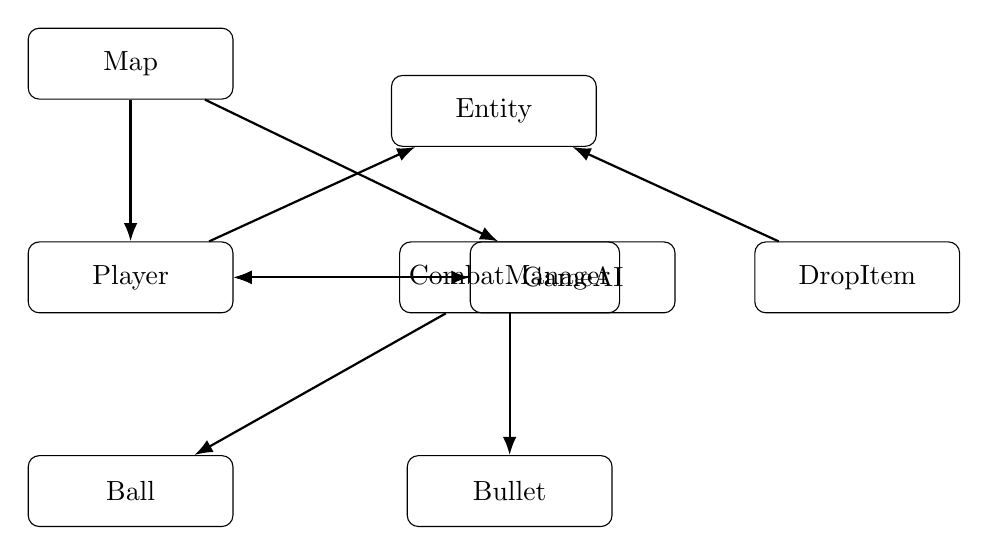
\begin{tikzpicture}[
  class/.style={rectangle, draw, rounded corners, align=center, minimum width=2.6cm, minimum height=0.9cm},
  rel/.style={-Latex, thick}
]
\node[class] (entity) {Entity};
\node[class, below left=1.2cm and 2.0cm of entity] (player) {Player};
\node[class, below right=1.2cm and 2.0cm of entity] (dropitem) {DropItem};
\node[class, right=3.0cm of player] (gameai) {GameAI};
\node[class, below=1.8cm of player] (ball) {Ball};
\node[class, right=2.2cm of ball] (bullet) {Bullet};
\node[class, above=1.8cm of bullet] (combat) {CombatManager};
\node[class, above=1.8cm of player] (map) {Map};

\draw[rel] (player) -- (entity);
\draw[rel] (dropitem) -- (entity);
\draw[rel] (gameai) -- (player);
\draw[rel] (combat) -- (player);
\draw[rel] (combat) -- (gameai);
\draw[rel] (combat) -- (ball);
\draw[rel] (combat) -- (bullet);
\draw[rel] (map) -- (player);
\draw[rel] (map) -- (gameai);
\end{tikzpicture}
\caption{最小化核心类关系图（性价比导向）。Entity为基类，Player与DropItem继承之。CombatManager、GameAI、Map分别负责战斗、AI、寻路。}
\label{fig:uml-minimal}
\end{figure}

\section{编译与运行结果}


本节仅保留简单的运行结果说明，真实的游戏演示由视频补充，视频见附件。

\textbf{编译环境}：

\begin{itemize}
  \item \textbf{操作系统}：Windows 10/11
  \item \textbf{编译器}：MinGW GCC 11.2.0
  \item \textbf{Qt版本}：Qt 6.5.3 LTS / Qt 6.9.0
  \item \textbf{构建系统}：CMake 3.29+、Ninja
\end{itemize}

\textbf{测试方式}：按功能逐项验证，输入与输出都留作占位，便于后续填入视频中的真实过程。

\begin{longtable}{p{0.22\textwidth}p{0.34\textwidth}p{0.26\textwidth}p{0.12\textwidth}}
\toprule
\textbf{测试项} & \textbf{输入} & \textbf{输出} & \textbf{结论} \\
\midrule
\endfirsthead
\toprule
\textbf{测试项} & \textbf{输入} & \textbf{输出} & \textbf{结论} \\
\midrule
\endhead
基础攻击力结算测试 & 设置基础攻击、通用加成、武器倍率与专精倍率 & 观察到最终伤害按乘区顺序稳定增长，日志数值与预期一致 & 成功 \\
远程武器倍率测试 & 切换实心球与枪械并固定其他条件 & 观察到实心球、枪械伤害按各自倍率区分，输出差异符合设计 & 成功 \\
定身受击增伤测试 & 在定身状态下触发命中 & 观察到受击增伤判定生效，最终伤害高于非定身状态 & 成功 \\
护甲减伤测试 & 提高防守方护甲并重复命中 & 观察到最终伤害按护甲减伤后置衰减，数值变化符合预期 & 成功 \\
无尽模式成长测试 & 长时间运行并让对手持续获得伤害提升 & 观察到敌方输出逐步上升，容错率下降，未出现低压循环 & 成功 \\
\bottomrule
\end{longtable}

\textbf{结论}：

上述测试项均按预期完成，功能输入与输出能够形成闭环，说明系统在主要功能路径上运行正常，且便于后续用视频材料补充具体调试过程。


\appendix

\section{AI决策流程（必选 图2）}
\begin{figure}[H]
\centering
\begin{tikzpicture}[
  node distance=1.1cm,
  box/.style={rectangle, draw, rounded corners, align=center, minimum width=3.2cm, minimum height=0.8cm},
  arr/.style={-Latex, thick}
]
\node[box] (sense) {感知环境};
\node[box, below=of sense] (state) {选择状态};
\node[box, below left=0.9cm and 1.6cm of state] (attack) {攻击};
\node[box, below=of state] (pickup) {拾取};
\node[box, below right=0.9cm and 1.6cm of state] (cast) {释放法术};
\node[box, below=2.0cm of state] (recover) {卡住脱困/重新定位};

\draw[arr] (sense) -- (state);
\draw[arr] (state) -- (attack);
\draw[arr] (state) -- (pickup);
\draw[arr] (state) -- (cast);
\draw[arr] (attack) -- (sense);
\draw[arr] (pickup) -- (sense);
\draw[arr] (cast) -- (sense);
\draw[arr] (state) -- (recover);
\draw[arr] (recover) -- (sense);
\end{tikzpicture}
\caption{AI决策流程（最小化可读版本）。}
\label{fig:ai-flow}
\end{figure}

\section{战斗结算流程（必选 图3）}
\begin{figure}[H]
\centering
\begin{tikzpicture}[
  node distance=1.0cm,
  box/.style={rectangle, draw, rounded corners, align=center, minimum width=3.8cm, minimum height=0.8cm},
  arr/.style={-Latex, thick}
]
\node[box] (event) {输入或碰撞事件};
\node[box, below=of event] (check) {命中判定与目标验证};
\node[box, below=of check] (damage) {伤害/硬直/反弹逻辑};
\node[box, below=of damage] (update) {更新血量、状态、冷却};
\node[box, below=of update] (feedback) {动画、音效、UI反馈};

\draw[arr] (event) -- (check);
\draw[arr] (check) -- (damage);
\draw[arr] (damage) -- (update);
\draw[arr] (update) -- (feedback);
\end{tikzpicture}
\caption{战斗结算流水线。}
\label{fig:combat-flow}
\end{figure}

\section{伤害计算详细流程（必选 图4）}
\begin{figure}[H]
\centering
\begin{tikzpicture}[
  node distance=0.95cm,
  box/.style={rectangle, draw, rounded corners, align=center, minimum width=3.5cm, minimum height=0.75cm},
  arr/.style={-Latex, thick}
]
\node[box] (hit) {碰撞有效};
\node[box, below=of hit] (attacker) {获取攻击者属性};
\node[box, below=of attacker] (defender) {获取防守者属性};
\node[box, below=of defender] (base) {基础伤害 = 武器伤害};
\node[box, below=of base] (burst) {触发暴击？Y增伤50\%};
\node[box, below=of burst] (modifier) {应用词条修饰};
\node[box, below=of modifier] (armor) {减去护甲减伤};
\node[box, below=of armor] (stagger) {计算硬直时间};
\node[box, below=of stagger] (reflection) {反弹判定};
\node[box, below=of reflection] (apply) {应用伤害与状态};

\draw[arr] (hit) -- (attacker);
\draw[arr] (attacker) -- (defender);
\draw[arr] (defender) -- (base);
\draw[arr] (base) -- (burst);
\draw[arr] (burst) -- (modifier);
\draw[arr] (modifier) -- (armor);
\draw[arr] (armor) -- (stagger);
\draw[arr] (stagger) -- (reflection);
\draw[arr] (reflection) -- (apply);
\end{tikzpicture}
\caption{伤害计算详细流程（含暴击、词条、护甲、硬直、反弹）。}
\label{fig:damage-calc}
\end{figure}

\end{document}
